\documentclass[tikz,border=3mm]{standalone}
\usepackage[T1]{fontenc}
\usepackage[utf8]{inputenc}
\usepackage{lmodern}
\usetikzlibrary{arrows.meta,positioning,calc,shapes.geometric}
\definecolor{ink}{HTML}{202A33}
\definecolor{blue}{HTML}{2D7F9D}
\definecolor{orange}{HTML}{C97728}
\definecolor{light}{HTML}{B0C0D0}
\definecolor{soft}{HTML}{F3F5F7}
\begin{document}
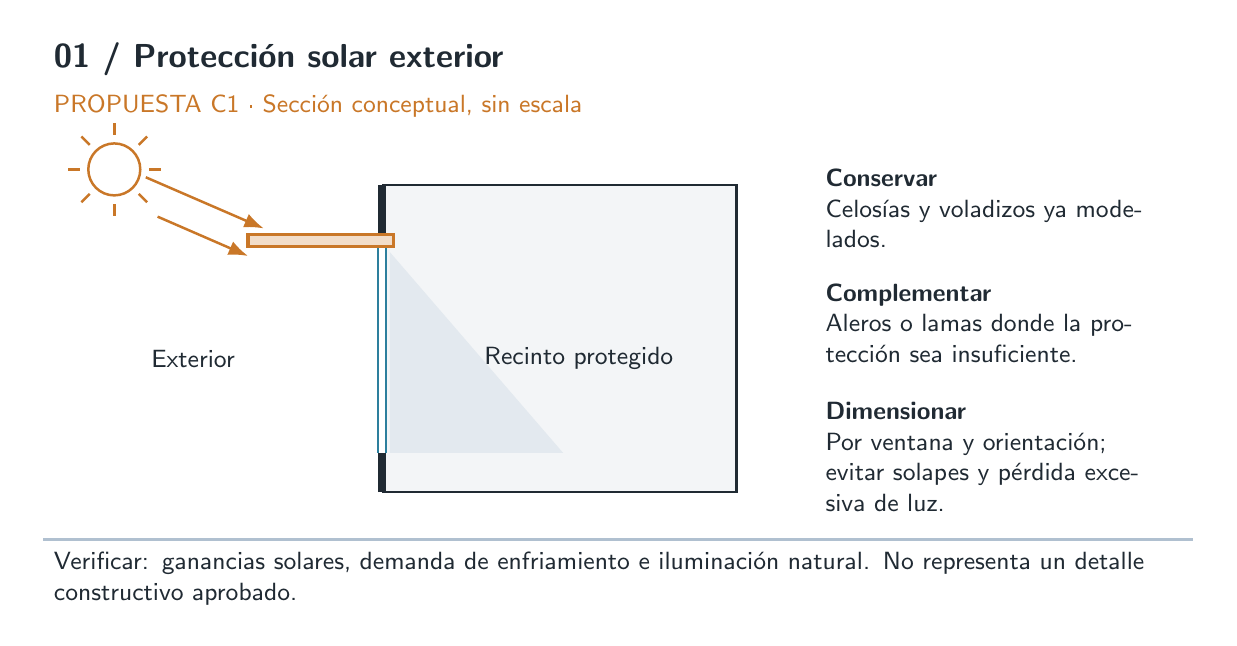
\begin{tikzpicture}[x=1cm,y=1cm,>=Latex,line width=.9pt,every node/.style={font=\sffamily\small,text=ink},note/.style={align=left,text width=4.1cm,anchor=west},flow/.style={->,blue,line width=1.2pt}]
\path[use as bounding box] (0,0) rectangle (15,7.5);

\node[anchor=west,font=\sffamily\bfseries\large] at (.2,7.1) {01 / Protección solar exterior};
\node[anchor=west,text=orange] at (.2,6.5) {PROPUESTA C1 · Sección conceptual, sin escala};
\fill[soft] (4.5,1.6) rectangle (9,5.5);
\draw[ink] (4.5,1.6)--(9,1.6)--(9,5.5)--(4.5,5.5);
\draw[ink,line width=3pt] (4.5,1.6)--(4.5,2.1) (4.5,4.7)--(4.5,5.5);
\draw[blue,double,double distance=2pt] (4.5,2.1)--(4.5,4.7);
\fill[orange!25] (2.8,4.72) rectangle (4.65,4.87);
\draw[orange,line width=1.2pt] (2.8,4.72) rectangle (4.65,4.87);
\fill[light!35] (4.6,4.65)--(6.8,2.1)--(4.6,2.1)--cycle;
\draw[orange] (1.1,5.7) circle (.33);
\foreach \a in {0,45,...,315} \draw[orange] (1.1,5.7)++(\a:.44)--++(\a:.15);
\draw[->,orange] (1.5,5.6)--(3,4.95);
\draw[->,orange] (1.65,5.1)--(2.8,4.6);
\node[align=center] at (2.1,3.3) {Exterior};
\node[align=center] at (7,3.3) {Recinto\ protegido};
\node[note] at (10,5.2) {\textbf{Conservar}\\Celosías y voladizos ya modelados.};
\node[note] at (10,3.75) {\textbf{Complementar}\\Aleros o lamas donde la protección sea insuficiente.};
\node[note] at (10,2.05) {\textbf{Dimensionar}\\Por ventana y orientación; evitar solapes y pérdida excesiva de luz.};
\draw[light] (.2,1)--(14.8,1);
\node[anchor=west,text width=14cm,align=left] at (.2,.5) {Verificar: ganancias solares, demanda de enfriamiento e iluminación natural. No representa un detalle constructivo aprobado.};

\end{tikzpicture}
\end{document}
